\section{Umsetzung: Methoden}
\subsection{Methoden zum Emotion Tracking}\label{MethodenEmotionTracking}
Es gibt verschiedene Methoden um die Emotion eines Nutzers während dessen Interaktion mit einer Maschine zu tracken. Im folgenden werden beispielhaft verschiedene Methoden erläutert:

\subsubsection{Hautwiderstand und Hauttemperatur}
Das Paper "A Suggestion to Improve User-Friendliness Based
on Monitoring Computer User’s Emotions" beschreibt, wie Emotionen eines Nutzers durch dessen Hauttemperatur und Hautwiderstand bestimmt werden können. Die Autoren nutzen dafür ein Temperatur- und Hautwiderstandssensor, die mit einem Arduino verbunden sind. Die Daten der Sensoren werden in einer SQLite Datenbank gespeichert und auf einer Android App ausgegeben. Die Autoren stellten fest, dass eine Änderung der Hauttemperatur bzw. des Hautwiderstands  auf eine Emotionsänderung des Nutzers zurückzuführen ist \cite{EmotionTrackingGSR}.

\subsubsection{Blick}
Die Autoren des Papers "Improving Human-Computer Interaction
by Gaze Tracking" untersuchten, wie das Tracken des Blickes des Nutzers zur Steuerung von Maschinen verwendet werden kann. Unter anderem konnte festgestellt werden, wo und wie lange der Nutzer ein Objekt auf der Maschine betrachtet. Dabei wurde festgestellt, dass durch dieses Verfahren auch die Emotionen eines Nutzers bestimmt werden können. Beispielsweise verändert sich die Pupillengröße bei einer Emotionsänderung des Nutzers. Dabei nutzen die Autoren die integrierte Webcam in einem Laptop, um den Blick und somit die Emotionen eines Nutzers zu Tracken. Somit wird keine zusätzliche Hardware benötigt, wenn das Endgerät des Nutzers bereits eine Kamera integriert hat \cite{EmotionTrackingGaze}.

\subsubsection{Gesichtsausdruck}
Cloud Service Anbieter wie Amazon, IBM und Microsoft bieten Cognitive Services an, darunter auch ein Service zur Emotionserkennung. Abbildung \ref{fig:microsoftgestenerkennung} zeigt eine Live Demo des Service von Microsoft, dabei wird die Emotion "Überraschung" mit einer Wahrscheinlichkeit von 0,93 erkannt. Bei der Live Demo kann ein Bild hochgeladen oder direkt wie Webcam aufgezeichnet werden. Der Service erkennt dann zuerst die Person bzw. Personen und bestimmt zu jeder Person, mit viel Prozent diese mit einer vorgegeben Emotionen übereinstimmt.

\begin{figure}[!h]
	\centering
	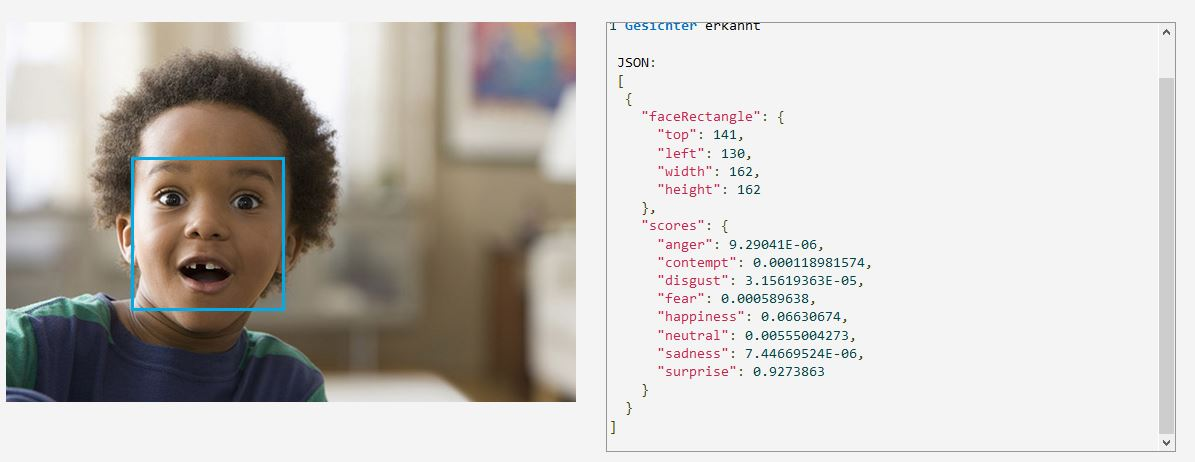
\includegraphics[width=0.9\linewidth]{Pictures/Microsoft_Gestenerkennung}
	\caption[Beispiel: Microsoft Azure Emotionserkennung]{Beispiel: Microsoft Azure Emotionserkennung \cite{MicrosoftAzure}}
	\label{fig:microsoftgestenerkennung}
\end{figure}

\subsubsection{Sprachinformationen}
Die Emotionen eines Menschen spiegeln sich in der Sprache dessen wieder. Ein typisches Beispiel hierfür ist, wenn eine Person einen Vortrag hält und dabei sehr verunsichert und aufgeregt ist, die Person spricht oft schnell und verspricht sich gegebenenfalls. Die Autoren des Papers "Speech emotion recognition approaches in human computer interactiong" untersuchten, wie genau können Emotionen eines Nutzers durch die Sprachinformationen bestimmt werden. Dabei extrahierten diese Muster aus mehreren Sprachsignal und bestimmten für dieses Muster die Emotionen des Sprechers. Diese Informationen wurden dann verwendet, um eine künstliche Intelligenz zu trainieren, um somit für ein beliebiges Sprachsignale die zugehörige Emotion vorherzusagen \cite{SpeechInformation}.

\subsection{Workshop Aufgabe}
Im Workshop wollten wir gemeinsam mit allen Teilnehmern so viele Methoden wie möglich zum Emotion Tracking finden. Dazu wurden die in Kapitel \ref{MethodenEmotionTracking} genannten Methoden den Teilnehmern erstmal vorenthalten. Die Aufgabe wurde folgendermaßen gestellt:

\begin{itemize}
	\item Gruppengröße: 4 Personen
	\item Bearbeitungszeit: 10 Minuten
	\item Arbeitsverfahren: Recherche
	\item Beschreibung: Recherchieren Sie im Internet über Methoden zum Tracken der Emotionen einer Person. Diskutieren Sie die Methode in Ihrer Gruppe und notieren Sie Ihre Ergebnisse in dem folgenden Google Formular.
\end{itemize}

\subsection{Workshop Ergebisse}

Es zeigt sich, dass die geplante Zeit für diese Aufgabe ausreichend war. Die Teilnehmer sammelten in den 10 Minuten 23 Methoden zum Emotionen Tracking. Es wurde ein Google Formular verwendet, da somit die gefunden Methoden übersichtlich und ohne großen Aufwand über den Beamer den Teilnehmer präsentiert werden konnten. Dabei wurden die Methoden einzeln durchgegangen, falls ein Name einer Methode nicht selbsterklärend war, wurde der Verfasser gebeten, die Funktionsweise der Methode kurz zu erklären. Im folgenden eine kurze Auflistung der Ergebnisse, die die Methoden aus Kapitel \ref{MethodenEmotionTracking} ergänzen:

\begin{itemize}
	\item Überwachung von Körperfunktionen
	\begin{itemize}
		\item Herzschlag
		\item Gehirnströme
		\item Atmung
		\item Muskelspannung
	\end{itemize}
	\item Eingabeverhalten auf dem Endgerät	
\end{itemize}

